\documentclass{article}
\usepackage{nips12submit_e,times}

\usepackage[square,numbers]{natbib}
\usepackage{amsmath,amsthm,amssymb,amsfonts,MnSymbol,epsfig,graphicx,algorithm,algorithmic}
\newcommand{\red}[1]{\textcolor{red}{\textsf{\emph{\textbf{\textcolor{red}{#1}}}}}}

\title{Dynamic Bayesian Gaussian Graphical Models for Inferring Evolving Network Structure}

\author{ % I've put alphabetical by last name
Slav Kirov\\
Dept. of Mathematical Sciences\\
Carnegie Mellon University\\
Pittsburgh, PA 15213 \\
\texttt{skirov@andrew.cmu.edu} \\
\And
Micol Marchetti-Bowick\\
School of Computer Science\\
Carnegie Mellon University\\
Pittsburgh, PA 15213 \\
\texttt{micolmb@cs.cmu.edu} \\
\And
Willie Neiswanger\\
School of Computer Science\\
Carnegie Mellon University\\
Pittsburgh, PA 15213 \\
\texttt{willie@cs.cmu.edu} \\
}

\newcommand{\fix}{\marginpar{FIX}}
\newcommand{\new}{\marginpar{NEW}}

\nipsfinalcopy % Comment this line for anonymous authors and rough-draft template

\begin{document}

\maketitle

\begin{abstract}
We propose a method for learning the structure of evolving Gaussian graphical models via Bayesian inference. Gaussian graphical models (GGMs) are often used to model the structure of a network, where they have found applications in biology (gene networks), finance (relationships among stocks), computer vision (object pose) and a number of related fields. Our dynamic model is able to learn the structure of GGMs up to 100 nodes, and can recover an evolving GGM with more accuracy than its static counterpart. We demonstrate the model on two real-world datasets.
\end{abstract}


\section{Introduction}
\label{sec:intro}

Learning the structure of a network is a problem of interest in a variety of fields. For a biologist, uncovering the structure of a gene network that charactarizes functional associations between genes can provide insight into how genes interact during the regulation of a biological process. 
Similarly, a financial analyst may be interested in understanding how the prices of different stocks relate to one another. 
In both of these settings, learning a dynamic network that evolves over time can provide even more valuable information about how these relationships vary under different conditions.
Inferring the structure of a dynamic gene network---such as one that evolves over the course of a biological lineage---can provide insight into how gene associations change as a cell differentiates. 
Learning a dynamic network of stocks as the market evolves over time can provide valuable information about which stocks co-vary and how these relationships are influenced by external factors.

A variety of approaches have been used in the past to model static networks with hidden structure. One of the most popular is the Gaussian Graphical Model (GGM), which assumes that a set of observations $X_1,...,X_n$ where $X_i \in \mathbb{R}^p$ are drawn IID from a multivariate normal distribution with mean $0$ and unknown covariance $\Sigma \in \mathbb{R}^{p \times p}$. The conditional indepenence relationships between variables are encoded in the precision matrix, $\Omega = \Sigma^{-1}$. If the ${ij}^{\text{th}}$ element of $\Omega$ is 0 then $X_i$ and $X_j$ are conditionally independent given all of the other variables. We can encode the (unweighted) conditional independence structure of this model in a graph, $G$, with $p$ nodes and an edge between node $X_i$ and node $X_j$ if and only if $\Omega_{ij} = 0$.

%Recently, many techniques have emerged for estimating the structure of the graph $G$ that encodes the conditional independence structure of a set of variables in a GGM. Two of the most popular approaches are neighborhood selection \cite{meinshausen2006high} and glasso \cite{friedman2008sparse}, both of which involve running a variant of Lasso regression, which uses an L1 penalty to encourage sparsity in the resulting graph. Although these discriminative methods are efficient for very large networks (over 1,000 nodes) and have good statistical guarantees, they lack the expressiveness and flexibility of generative models.

%A few approaches have been developed for formulating the GGM as a generative model and performing Bayesian inference to estimate the structure of the underlying graph. Although some of these have proven successful as well, their main drawback is that they are only efficient for much smaller networks (under 100 nodes). In many cases, however, generative models have advantages over discriminative techniques because they can more easily be extended to incorporate both prior knowledge and additional observations from new data sources. 

Here, we propose a generative model for a time-evolving network. The model, which we call a Dynamic Bayesian Gaussian Graphical Model (DB-GGM), is constructed using a formulation of the GGM as a Bayesian network model that has been developed in the past for a static network. By introducing a dependence between the underlying graph at each time point, we convert the static model into a dynamic Bayesian network. We then derive two Bayesian inference procedures for our model, and evaluate their performance on a synthetic dataset. Finally, we apply our method to two real datasets: a gene network that encodes relationships between the activity levels of genes, and a network of stocks that encodes relationships between stock prices.

\subsection{Previous Work}
\label{sec:prev-work}
%There has much prior work for methods of inferring networks. One group of approaches involves using block structures as priors for graphs. Mansingha et al, 2006 \cite{mansinghka2006structured}, assume nodes in a Bayesian network come in one or more classes, and that prior probabilities of edges existing between two nodes depend only on their classes. Inference is done by an MCMC method consisting of moves on graphs, and moves on the latent states that describe the blockstructure. Marlin and Murphy, 2009 \cite{marlin2009sparse}, use a similar modeling approach in estimating sparse block-structured precision matrices. [more on that paper here]

%Parikh et al., 2011 \cite{parikh2011treegl}, estimate networks along a biological lineage using a Gaussian graphical model and perform inference via linear regression with both an $l_1$ and total variation penalty. KELLER (Song et al., 2009) \cite{song2009keller}, estimate time-varying interactions of genes between by using MRF model at each time step, and using logistic regression with a smoothing kernel, to recover networks that change gradually over time. 

%A class of approaches more related to our method involves using G-Wishart prior distributions of precision matrices of GGM's. Wang and Li, 2012 \cite{wang2012efficient}, develope an MCMC sampling procedure for learning a Gaussian graphical model. A related birth-death MCMC inference approach is employed by Mohammadi and Wit \cite{mohammadi2012efficient}.

Recently, many techniques have emerged for estimating the structure of the graph $G$ that encodes the conditional independence structure of a set of variables in a static GGM. Two of the most popular approaches are neighborhood selection \cite{meinshausen2006high} and glasso \cite{friedman2008sparse}, both of which involve running a variant of Lasso regression, which uses an L1 penalty to encourage sparsity in the resulting graph. Although these discriminative methods are efficient for very large networks (over 1,000 nodes) and have good statistical guarantees, they lack the expressiveness and flexibility of generative models.

A few approaches have been developed for formulating a static GGM as a generative model and performing Bayesian inference to estimate the structure of the underlying graph. In many cases, though only efficient for relatively small networks (under 100 nodes), generative models have advantages over discriminative techniques because they can more easily be extended to incorporate both prior knowledge and additional observations from new data sources \cite{roverato2002hyper,jones2005experiments,green1995reversible}. A class of these approaches involves using G-Wishart prior distributions for precision matrices of GGM's. Wang and Li, 2012 \cite{wang2012efficient}, develope an MCMC sampling procedure for inference in such a model, while a related birth-death MCMC inference approach is employed by Mohammadi and Wit \cite{mohammadi2012efficient}.

Finally, some methods have been proposed for estimating the structure of a network that evolves over time. Parikh et al. \cite{parikh2011treegl} estimate networks that evolve over a biological lineage using an evolving GGM and perform inference by extending neighborhood selection to penalize differences between adjacent networks. In KELLER, Song et al. \cite{song2009keller} estimate time-varying interactions of genes between by using MRF model at each time step and using logistic regression with a smoothing kernel to recover networks that change gradually over time.

\section{Methods}
\label{sec:methods}

In this section, we will discuss our model and inference procedures.

\subsection{Model}
\label{sec:model}
Our generative model is a dynamic Bayesian network (DBN) that incorporates a Gaussian graphical model (GGM) at each time step. The model consists of hidden variables $\{A_t\}_{t=1}^T$ and $\{K_t\}_{t=1}^T$ and observed variables $\{X_t\}_{t=1}^T$. $A_t = \{ A_{ij}^t : i < j \}$ is a $p\text{-by-}p$ adjacency matrix that represents the graph structure at time $t$. $K_t$ is a precision matrix for a multivariate Normal distribution with covariance $\Sigma_t = K_t^{-1}$. $K_t \mid A_t$ is drawn from a G-Wishart distribution, which is the conjugate prior for the distribution of a precision matrix of a GGM given a graph structure. $X_t$ is a vector $\in \mathbb{R}^p$ that is drawn from a multivariate Normal distribution with mean $0$ and covariance $\Sigma_t$. At time $t$, each $A_{ij}^t$ has a value of either 1 (edge present) or 0 (edge not present). The distribution of $A_{ij}^t$ depends on the value of the same edge at the previous time point. Each edge has a ``flip on'' and ``flip off'' probability, given by $p_{ij}^0$ and $p_{ij}^1$, respectively. These probabilities are defined as follows: 

\begin{align*}
p_{ij}^0 = P(A_{ij}^t = 1 \mid A_{ij}^{t-1} = 0) \hspace{.5in} 1 - p_{ij}^0 = P(A_{ij}^t = 0 \mid A_{ij}^{t-1} = 0) \\
p_{ij}^1 = P(A_{ij}^t = 0 \mid A_{ij}^{t-1} = 1) \hspace{.5in} 1 - p_{ij}^1 = P(A_{ij}^t = 1 \mid A_{ij}^{t-1} = 1)
\end{align*}

\begin{figure*}[tbp]
\centering
  \begin{minipage}[c]{0.6\linewidth}
      \centering               
      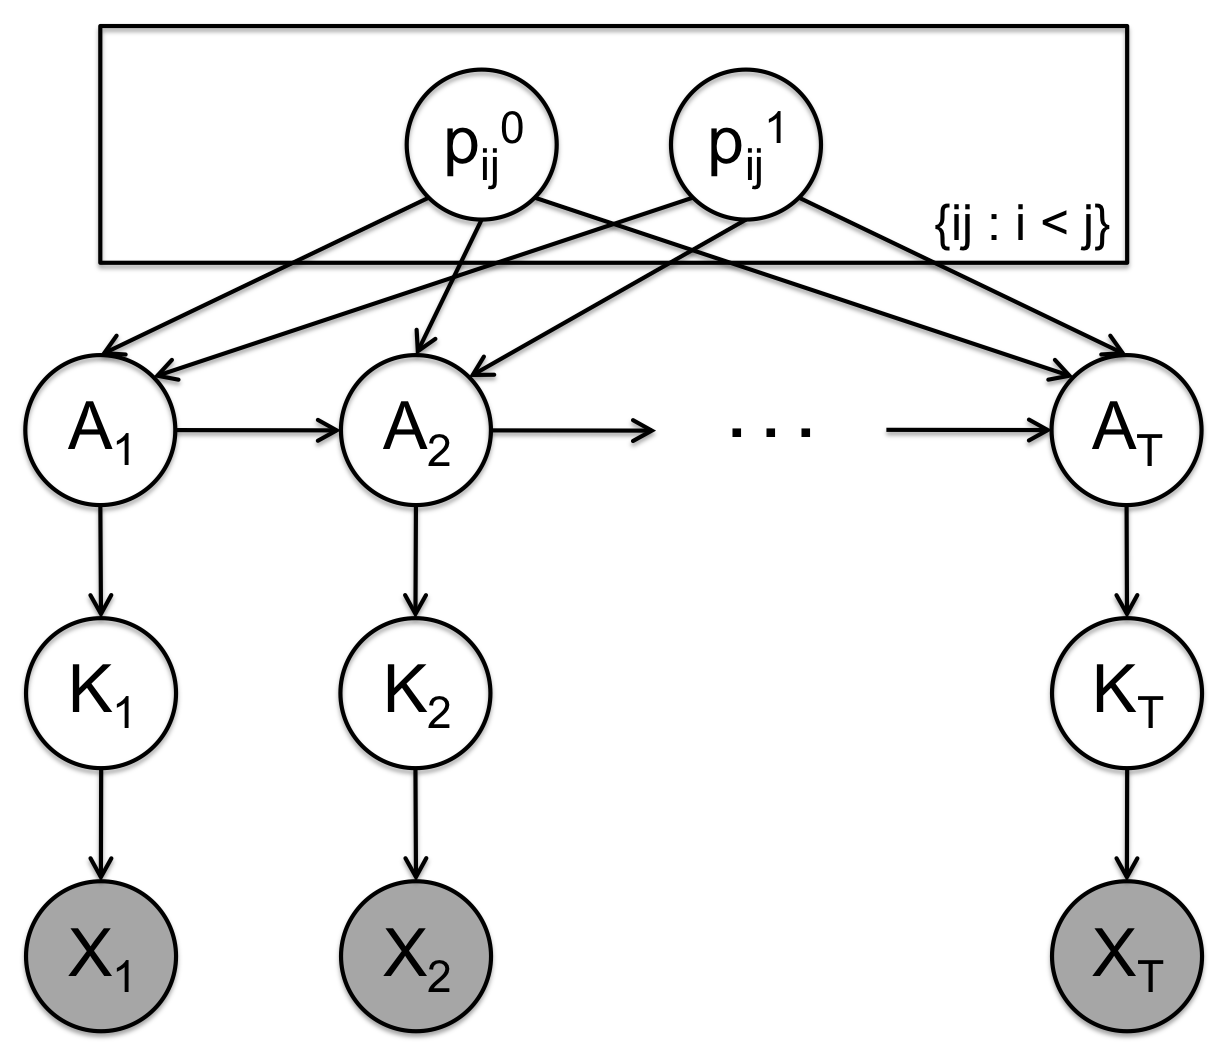
\includegraphics[width=0.8\textwidth]{fig/dynamic_ggm_model.png}
      \caption{Illustration of the graphical model for our dynamic Bayesian network. Note that each edge $A_{ij}^t$ only depends on one Bernoulli parameter, $p_{ij}^{a}$, given that its predecessor $A_{ij}^{t-1} = a$.}
      \label{fig:dynamicModel}
  \end{minipage}
  \hspace{0.05\linewidth}
  \begin{minipage}[c]{0.24\linewidth}
      \centering               
      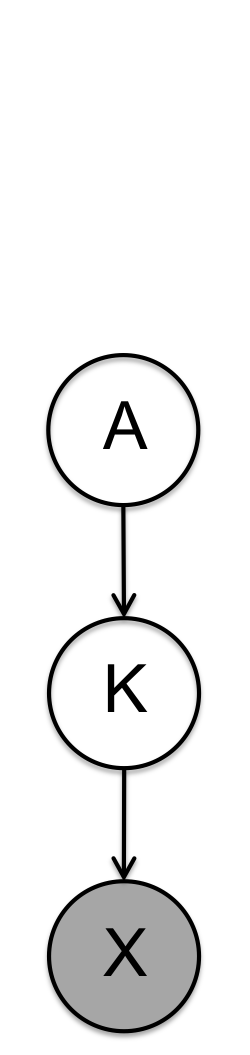
\includegraphics[width=0.4\textwidth]{fig/static_ggm_model.png}
      \caption{Illustration of the graphical model for the static counterpart to our Bayesian network.}
      \label{fig:staticModel}
  \end{minipage}
\end{figure*}

The specific parameterization of our model is given below and a depiction of the graphical model is provided in Figure \ref{fig:dynamicModel}. Note that the values of parameters $\alpha_0$, $\beta_0$, $\alpha_1$, $\beta_1$, $b$, and $D$ are set manually.

\begin{align*}
p_{ij}^0 &\sim \text{Beta}(\alpha^0,\beta^0) \\
p_{ij}^1 &\sim \text{Beta}(\alpha^1,\beta^1) \\
A_{ij}^t \mid (A_{ij}^{t-1} = 0) &\sim \text{Bernoulli}(p_{ij}^0) \\
A_{ij}^t \mid (A_{ij}^{t-1} = 1) &\sim \text{Bernoulli}(p_{ij}^1) \\
K_t \mid A_t &\sim \text{G-Wishart}_{A_t}(b,D) \\ 
X_t \mid K_t &\sim \text{Normal}(0,K_t^{-1})
\end{align*}

%\begin{align*}
%p_{ij}^0 \sim \text{Beta}(\alpha^0,\beta^0) &\hspace{.5in} p_{ij}^1 \sim \text{Beta}(\alpha^1,\beta^1) \\
%A_{ij}^t \mid (A_{ij}^{t-1} = 0) \sim \text{Bernoulli}(p_{ij}^0) &\hspace{.5in} A_{ij}^t \mid (A_{ij}^{t-1} = 1) %\sim \text{Bernoulli}(p_{ij}^1) \\
%K_t \mid A_t \sim \text{G-Wishart}_{A_t}(b,D) &\hspace{.5in} X_t \mid K_t \sim \text{Normal}(0,K_t^{-1})
%\end{align*}

\subsection{Inference}
\label{sec:inference}
A number of previous works have focused on developing inference methods for a static Bayesian GGM such as the one shown in Figure \ref{fig:staticModel}, which is the direct static analog to the dynamic model we described in the previous section.

Most recently, Mohammadi and Wit \cite{mohammadi2012efficient}, proposed a technique called Birth-Death MCMC (BD-MCMC) for jointly sampling the graph structure $A$ and the precision matrix $K$ in order to infer the posterior $P(A,K \mid X)$. Briefly, BD-MCMC involves constructing a Markov chain whose stationary distribution is $P(A,K \mid X)$ by formulating it as a birth-death process, where each state corresponds to a graph with a specific number of edges, $E$, and its associated precision matrix. The transition probabilities are encoded as birth rates and death rates, and it is the specification of these rates which determines the stationary distribution. Inference is performed by traversing the space of possible assignments to the hidden variables by executing birth moves (adding an edge) and death moves (removing an edge) and resampling the precision matrix after each move. Sampling the precision matrix from a G-Wishart distribution is done by relying on properties of the Choleski Decomposition of the precision matrix. BD-MCMC runs efficiently on graphs with up to 100 nodes.

\begin{algorithm}[h!tbp]
\caption{Birth-Death MCMC}
\label{alg:j}
\begin{algorithmic}[1]
\STATE \textbf{inputs:} Data $X$ and prior on adjacency matrices $P(A)$
\STATE Initialize A as an upper triangular matrix with all ones
\STATE Sample precision matrix K
\STATE Define birth rates $\beta_{(i,j)}(K) = 1$ for all $(i,j) \in \bar{E} := \{(i,j): i \leq j, A_{(i,j)} = 0\}$
\REPEAT 
\STATE Calculate the total birth rate $\beta(K) = |\bar{E}|$ 
\STATE Calculate the death rates, $$\delta_{(i,j)}(K) = \frac{p(X \mid K_{-(i,j)},A_{-(i,j)})p(A_{-(i,j)})}{p(X \mid K,A)p(A)}, \quad \text{for all }(i,j) \in \bar{E}$$
\STATE Calculate the total death rate, $\delta(K) = \sum_{(i,j) \in E} \delta_{(i,j)}(K)$
\STATE Calculate the waiting time, $\lambda(K) = \beta(K)+\delta(K)$
\STATE Simulate the type of jump (birth or death), with respective probabilities: $$ p(\text{birth of } (i,j)) = \frac{\beta_{(i,j)}(K)}{\lambda(K)}, \quad \text{for all } (i,j) \in \bar{E}$$ $$ p(\text{death of } (i,j)) = \frac{\delta_{(i,j)}(K)}{\lambda(K)}, \quad \text{for all } (i,j) \in E$$
\IF{birth of $(i,j)$} Sample a new precision matrix $K \text{ given } A_{+(i,j)}$ 
\ELSIF{death of $(i,j)$} Sample a new precision matrix $K \text{ given } A_{-(i,j)}$
\ENDIF
\UNTIL{convergence}
\STATE \textbf{output:} Samples from the full posterior distribution, $P(A,K \mid X)$
\end{algorithmic}
\label{alg:smc}
\end{algorithm}

Here, we build on prior work to derive an inference method for the dynamic Bayesian GGM described in Section \ref{sec:model}. We experiment with two different inference procedures: Sequential Monte Carlo (SMC) and collapsed Gibbs sampling, a type of MCMC. 

\subsubsection{Sequential Monte Carlo}

SMC is a type of inference that is well suited for dynamic models, as it performs Bayesian inference in an online manner. Here, it is particularly useful because it allows us to build upon a previously established inference technique (BD-MCMC) for approximating the partial posterior distribution at each time step.

SMC works in the following way. At time $t-1$, we assume we have $N$ particles (samples of $A_{1:t-1}$ and $K_{1:t-1}$) that are approximately sampled from the posterior distribution $P(A_{1:t-1},K_{1:t-1} \mid X_{1:t-1})$. We then want to update these particles at time $t$ so that we end up with $N$ particles approximately sampled from $P(A_{1:t},K_{1:t} \mid X_{1:t})$. In this way, after we've gone through every time step, we will end up with $N$ samples from the full posterior distribution, $P(A_{1:T},K_{1:T} \mid X_{1:T})$. The SMC algorithm that we derived is outlined in Algorithm \ref{alg:smc}. 

\begin{algorithm}[h!tbp]
\caption{SMC for Dynamic Bayesian GGM}
\label{alg:smc}
\begin{algorithmic}[1]
\STATE \textbf{inputs:} \\(i) A sequence of observations $X_t : t = 1,...,T$ \\(ii) Parameters $b$ and $D$ for the G-Wishart prior over precision matrices \\(iii) Parameters $\alpha^0$, $\beta^0$, $\alpha^1$, $\beta^1$ for the Beta priors over the Bernoulli parameters $p_{ij}^0$ and $p_{ij}^1$ \\(iv) Number of particles, $N$
\STATE Run BD-MCMC using data $X_1$ and uniform graph prior $P(A_{1})$ as inputs; outputs samples from the partial posterior distribution $P(A_1,K_1 \mid X_1)$
\STATE Generate $N$ particles sampled from $P(A_1,K_1 \mid X_1)$
\FOR{$t = 2,...,T$}
\FOR{$i = 1,...,N$}
\STATE Sample $A_t$ and $K_t$ from the proposal distribution, $$Q_t(A_t,K_t \mid A_{1:t-1}^{(i)},K_{1:t-1}^{(i)},X_{1:t})$$ using BD-MCMC with data $X_{t}$ and graph prior $P(A_{t}) = P(A_{t}|A_{t-1})$ as inputs.
\STATE Extend particle $i$ with $A_t$ and $K_t$
\STATE Evaluate the importance weight, $$w_t^{(i)} \propto \frac{P(X_t \mid A_t^{(i)}, K_t^{(i)}) P(A_t^{(i)}, K_t^{(i)} \mid A_{1:t-1}^{(i)}, K_{1:t-1}^{(i)}, X_{1:t-1})}{Q_t(A_t,K_t \mid A_{1:t-1}^{(i)},K_{1:t-1}^{(i)},X_{1:t})}$$
\ENDFOR
\STATE Resample the particles according to a categorical distribution made up of the normalized weights $w_1,...,w_N$
\ENDFOR
\STATE \textbf{output:} $N$ samples from the full posterior distribution, $P(A_{1:T},K_{1:T} \mid X_{1:T})$
\end{algorithmic}
\label{alg:smc}
\end{algorithm}

For the proposal distribution in step 6, we use: 
$$Q_t = P(A_t, K_t \mid A_{1:t-1}^{(i)},K_{1:t-1}^{(i)},X_{1:t-1}) = P(A_t, K_t \mid K_{t-1}^{(i)}, A_{t-1}^{(i)}, X_{t}^{(i)})$$
%$$Q_t = P(A_t, K_t \mid A_{1:t-1}^{(i)},K_{1:t-1}^{(i)},X_{1:t-1}) = P(A_t, K_t \mid A_{t-1}) = P(K_t \mid A_t) P(A_t \mid A_{t-1})$$
%\begin{align*}
%Q_t(A_t,K_t \mid A_{1:t-1}^{(i)},K_{1:t-1}^{(i)},X_{1:t}) &= P(A_t, K_t \mid A_{1:t-1}^{(i)},K_{1:t-1}^{(i)},X_{1:t-1}) \\
%&= P(A_t, K_t \mid A_{t-1}) \\
%&= P(K_t \mid A_t) P(A_t \mid A_{t-1})
%\end{align*}

To sample from $Q_t$, we carry out BD-MCMC with data $X_t$ and choose graph prior $P(A_{t}) = P(A_{t}|A_{t-1})$ (given in Section~\ref{sec:model}).

\subsubsection{Collapsed Gibbs Sampling}

Gibbs sampling is a type of MCMC that uses the conditional probability of a single variable conditioned on all other variables as the sampling distribution for that variable. In collapsed Gibbs sampling, some variables are integrated out so that they don't need to be sampled. Here, we integrate out $K_1,...,K_T$ and sample all other hidden variables. To do this, we iterate through all edges at each time step and sample new values for $A_{ij}^t$ from 

\begin{align*}
P(A_{ij}^t \mid \text{rest} \backslash K_{1:T}) &= P(A_{ij}^t \mid A_{-t}, A_{-ij}^t, X_{1:T}) \\
&= P(A_{ij}^t \mid A_{ij}^{t-1} A_{-ij}^t, A_{ij}^{t+1}, X_t) \\
%&= \frac{P(A_{ij}^{t-1}, A_{ij}^t, A_{-ij}^t, A_{ij}^{t+1}, X_t)}{\sum_{A_{ij}^t}P(A_{ij}^{t-1}, A_{ij}^t, A_{-ij}^t, A_{ij}^{t+1}, X_t)} \\
&= \frac{1}{Z} P(A_{ij}^t \mid A_{ij}^{t-1}) P(A_{ij}^{t+1} \mid A_{ij}^t) P(X_t \mid A_t) \\
&= \frac{1}{Z} P(A_{ij}^t \mid A_{ij}^{t-1}) P(A_{ij}^{t+1} \mid A_{ij}^t) \int_{K_t} P(X_t, K_t \mid A_t) \hspace{0.1cm} \mathrm{d} K_t \\
&= \frac{1}{Z} P(A_{ij}^t \mid A_{ij}^{t-1}) P(A_{ij}^{t+1} \mid A_{ij}^t) \int_{K_t} P(X_t \mid K_t) P(K_t \mid A_t) \hspace{0.1cm} \mathrm{d} K_t \\
&= \frac{1}{Z} P(A_{ij}^t \mid A_{ij}^{t-1}) P(A_{ij}^{t+1} \mid A_{ij}^t) (2\pi)^{(\frac{-np}{2})} \frac{I_{G[A_t]}(b+n, D+S)}{I_{G[A_t]}(b, D)}
\end{align*}

In the last line above, $I_{G[A_t]}$ is the normalization constant for a G-Wishart distribution with the given parameters that is consistent with graph $A_t$. $I_{G[A_t]}(b,D)$ is the normalization constant for the prior distribution over $K_t$ and $I_{G[A_t]}(b+n,D+S)$ is the normalization constant for the posterior distribution over $K_t \mid X_t$, where $n$ is the number of samples of $X_t$ and $S = X_t X_t^T$ is the sample covariance matrix of $X_t$. Although $I_G$ cannot be computed exactly, various approximations have been derived. Here we use a Monte Carlo simulation technique presented in \cite{ataykayismassam} to approximate $I_G$. For completeness, the Gibbs sampling algorithm that we use is outlined in Algorithm \ref{alg:gibbs}.

\begin{algorithm}[h!tbp]
\caption{Collapsed Gibbs Sampling for Dynamic Bayesian GGM}
\label{alg:gibbs}
\begin{algorithmic}[1]
\STATE \textbf{input:} \\(i) A sequence of observations $X_t : t = 1,...,T$ \\(ii) Parameters $b$ and $D$ for the G-Wishart prior over precision matrices \\(iii) Parameters $\alpha^0$, $\beta^0$, $\alpha^1$, $\beta^1$ for the Beta priors over the Bernoulli parameters $p_{ij}^0$ and $p_{ij}^1$ % \\(iv) Number of iterations $N$
\STATE Initialize values of and $A_{1:T}$
\WHILE {not converged}
\FOR {$t = 1,...,T$}
\FOR{$\{i,j\} : i < j$}
\STATE Sample a new value for $A_{ij}^t$ from $P(A_{ij}^t \mid \text{rest} \backslash K_{1:T})$
\ENDFOR
\ENDFOR
\ENDWHILE
\STATE \textbf{output:} Samples from the full posterior distribution, $P(A_{1:T} \mid X_{1:T})$
\end{algorithmic}
\label{alg:gibbs}
\end{algorithm}

\section{Experiments}
\label{sec:exp}

We carry out experiments on three data sets: synthetic data, stock data, and gene data taken from a lineage of stem cells.

\subsection{Synthetic Data}
We generate a synthetic sequence of 10 networks, and the corresponding observations in the following way. The first five graphs are all the same, where the first graph is generated randomly. The sixth graph exhibits additions or removals of a small number of edges in a Bernoulli fashion, and the remaining four graphs remain the same. Given a graph, we deterministically choose a consistent precision matrix $K_t$. Then we generate the observations $X_t \sim Normal(0,K_t))$.

We show preliminary results for a synthetically generated time-evolving network in Figure~\ref{fig:errorVsParticles}. This figure shows the number of incorrectly inferred edges vs number of particles for a 12-node graph varying over 10 time-steps. We also intend to demonstrate convergence of the sampler, and how both algorithm speed and performance changes with the number of observations, time-steps, and nodes.

\begin{figure*}[h!tbp]
  \centering               
  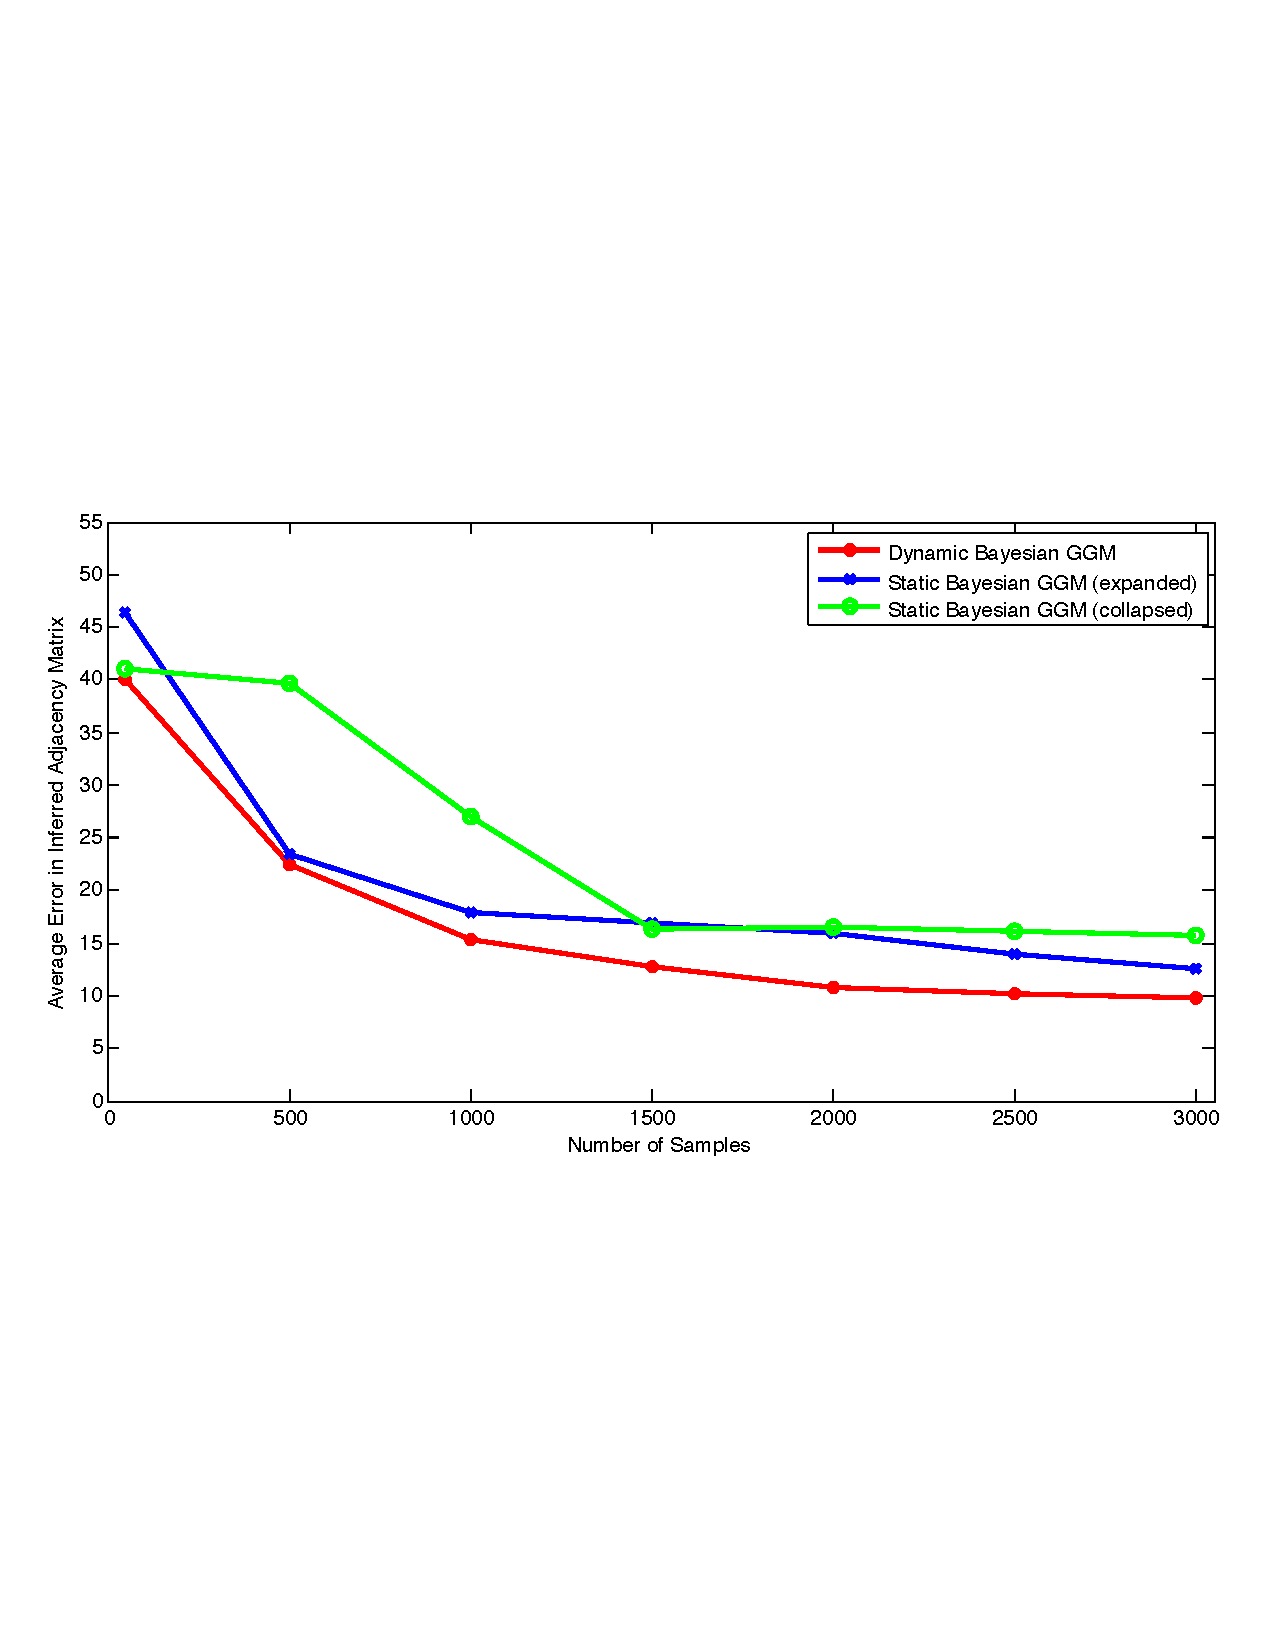
\includegraphics[width=0.9\textwidth]{fig/smcError.pdf}
  \caption{Average number of incorrectly inferred edges vs number of particles for the SMC inference algorithm. Each plotted point is an average over five runs.}
  \label{fig:errorVsParticles}
\end{figure*}

\begin{figure*}[h!tbp]
  \centering               
  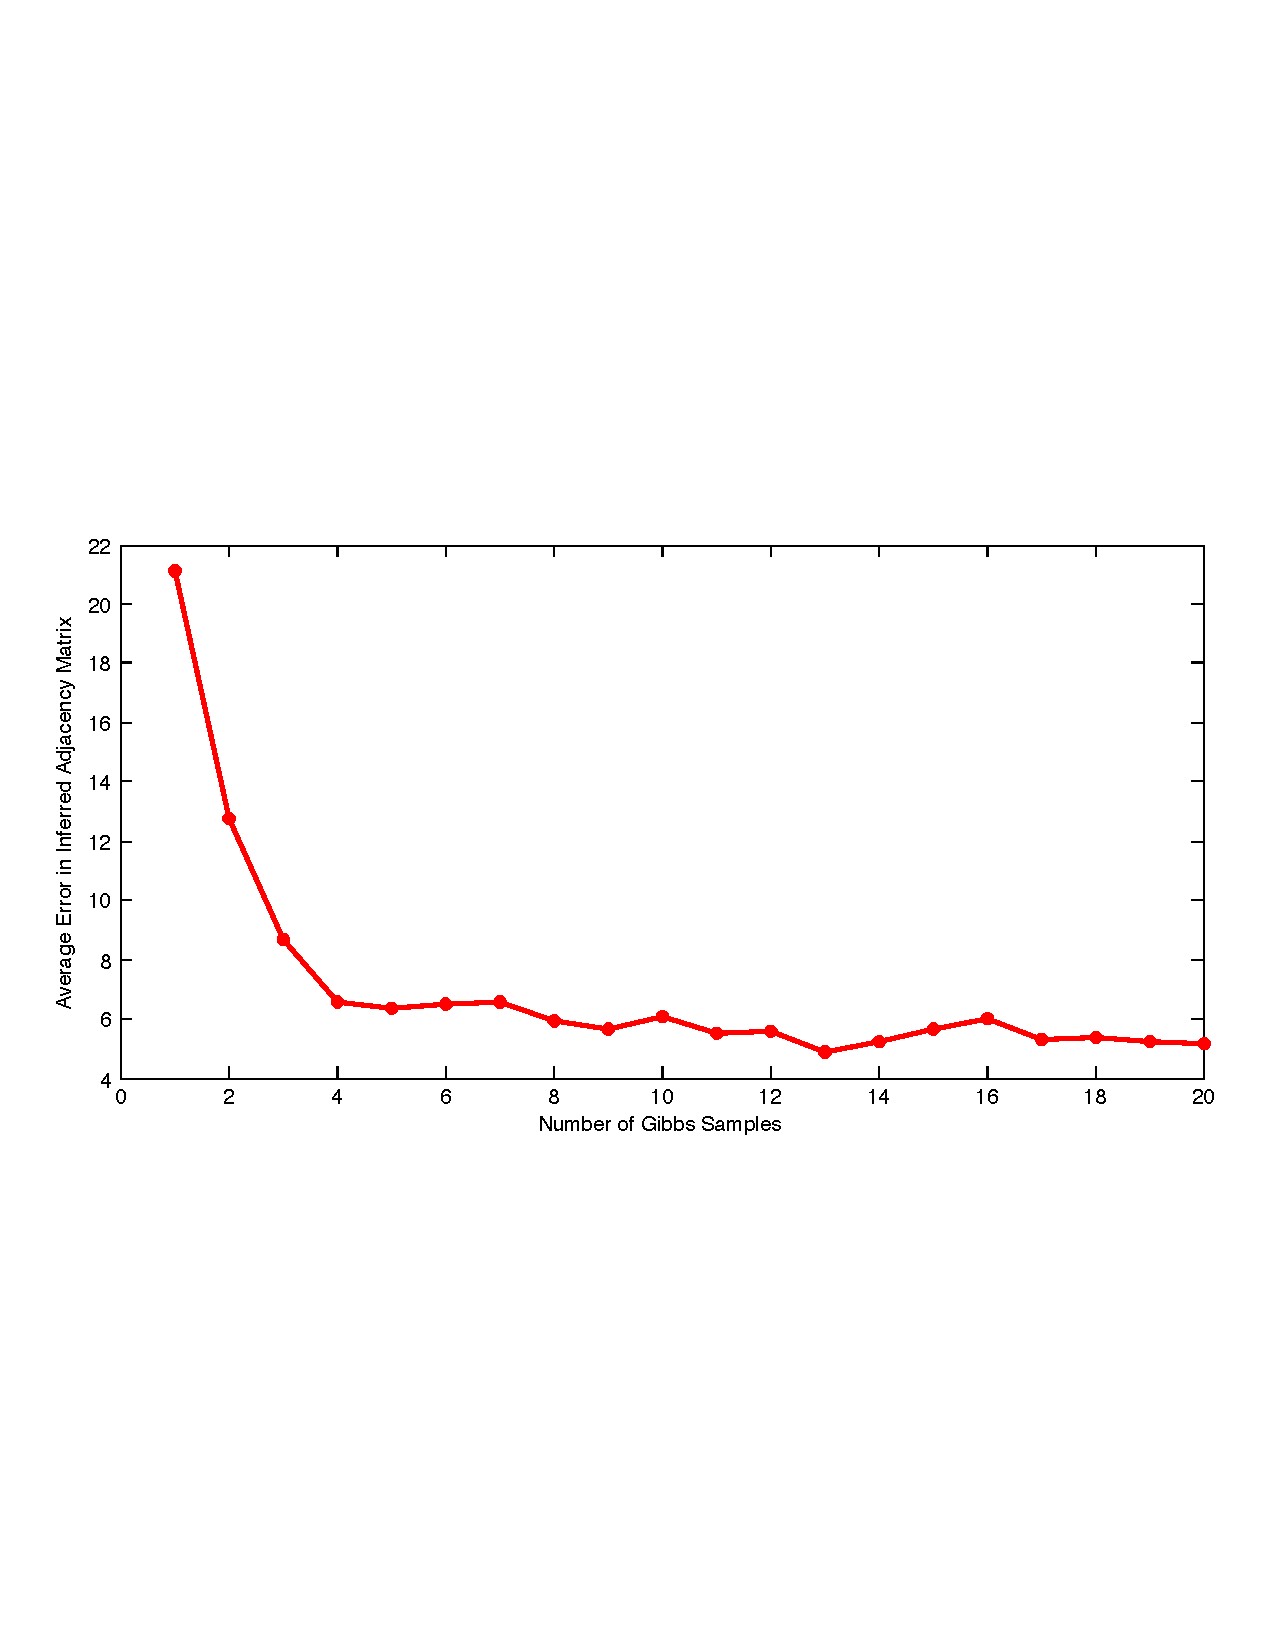
\includegraphics[width=0.9\textwidth]{fig/gibbsError.pdf}
  \caption{Average number of incorrectly inferred edges vs number of Gibbs iterations for the Gibbs inference algorithm. Each plotted point is an average over five runs.}
  \label{fig:errorVsSamples}
\end{figure*}

% Things to include:
% * Show convergence
% * Show how performance (accuracy) changes w/ number of observations
% * Show how performance (accuracy) changes w/ number of particles
% * Show how performance (accuracy) changes w/ number of time steps
% * Show how performance (accuracy) changes w/ number of nodes in graph
% * Show how performance (speed) changes w/ number of nodes in graph
% * Compare performance of static and dynamic case

\subsection{Genetic Networks}
In this experiment, we aim to infer a collection of gene networks in a lineage of cells. We hope the inferred networks will shed light on relations between the functions of groups of genes, and how these functions change as the underlying cells vary.

\begin{figure*}[h!tbp]
  \centering               
  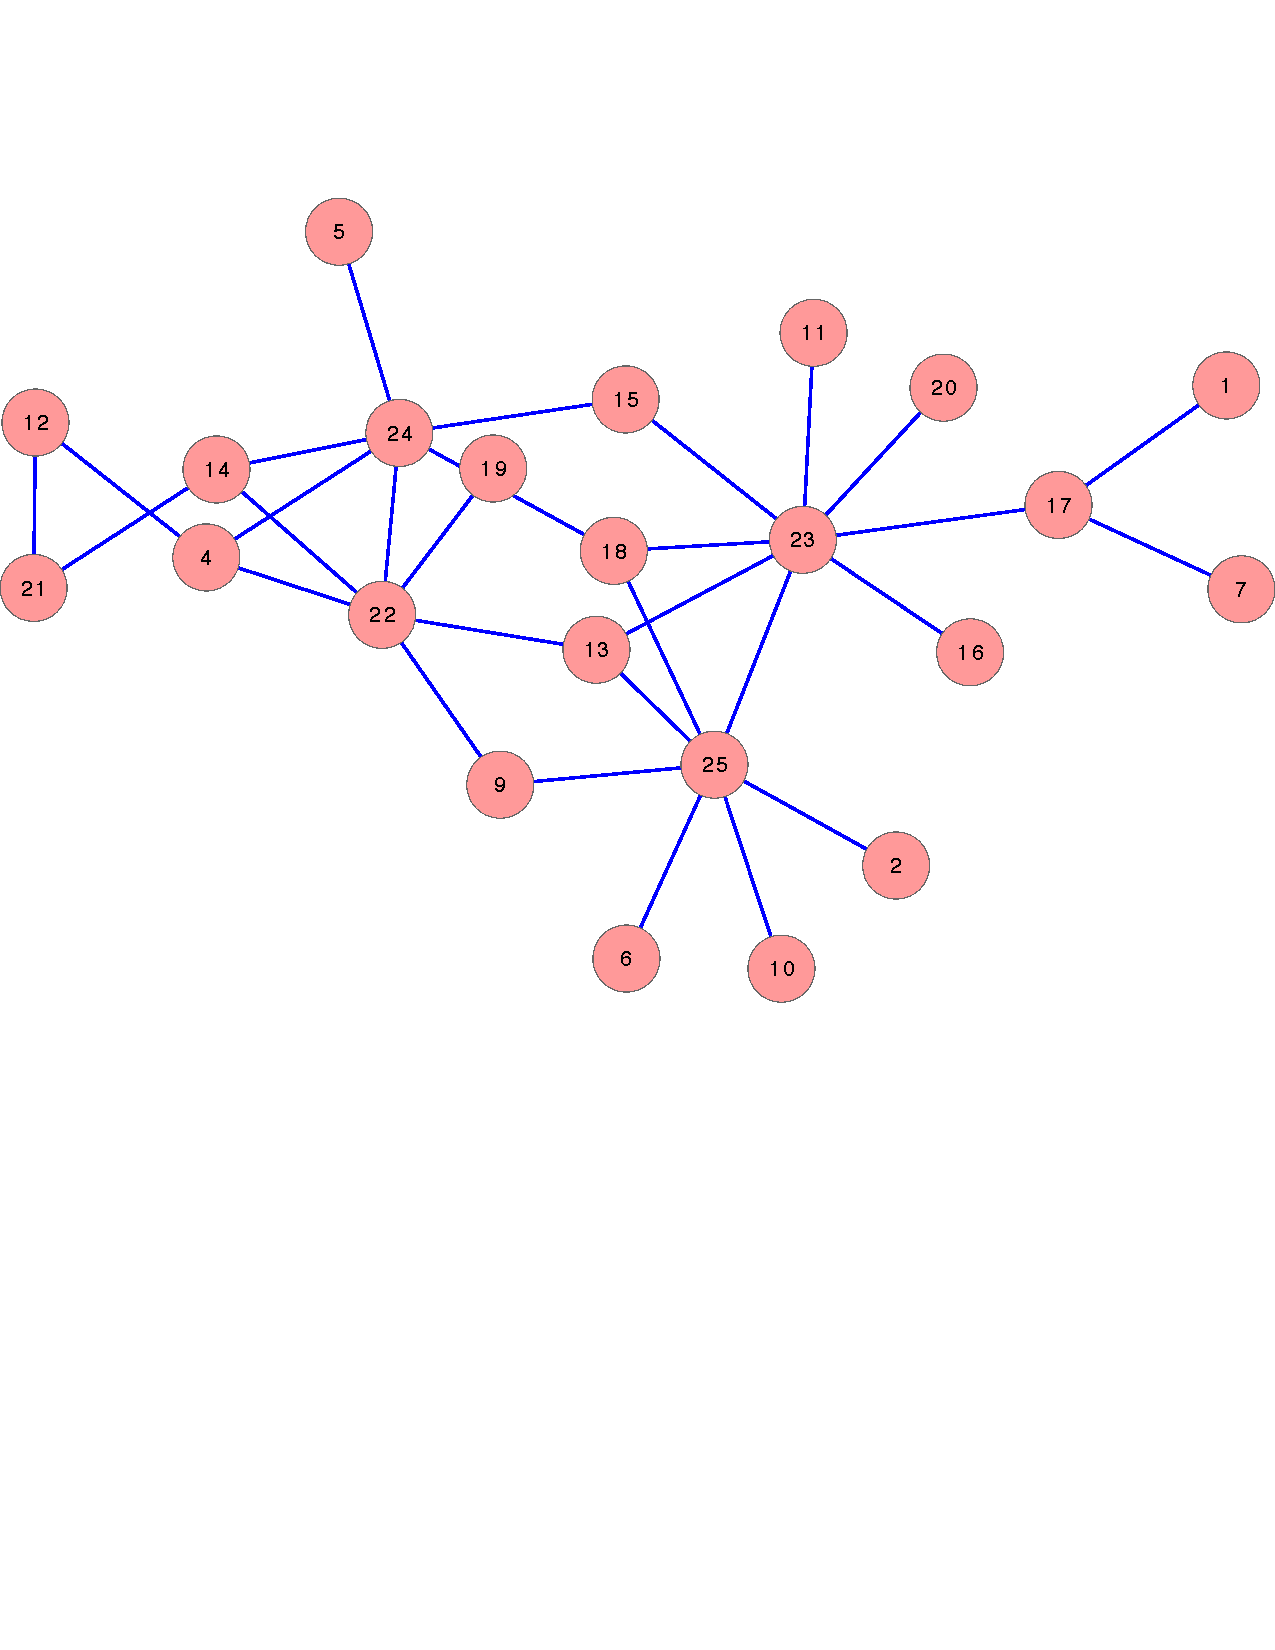
\includegraphics[width=0.8\textwidth]{fig/overallg3.pdf}
  \caption{Genetic network constructed by taking union over 9 inferred cell types}
  \label{fig:geneResults}
\end{figure*}


\subsection{Stock Market}
In this experiment, we aim to infer the network of time-varying relationships among a set of stocks. We hope the inferred network will give insight into related corporations based on the dynamics of their stock prices.

\begin{figure*}[h!tbp]
  \centering               
  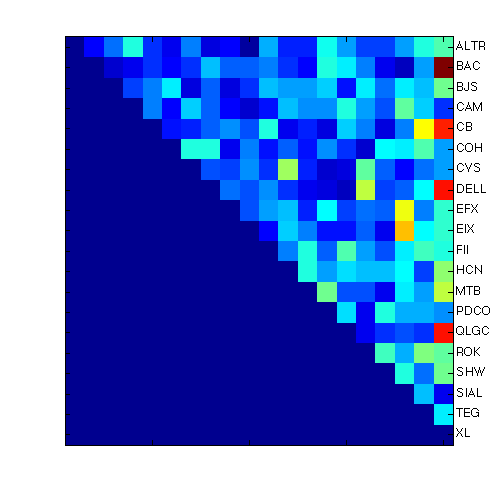
\includegraphics[height=0.18\textheight]{fig/stocks1.png}
  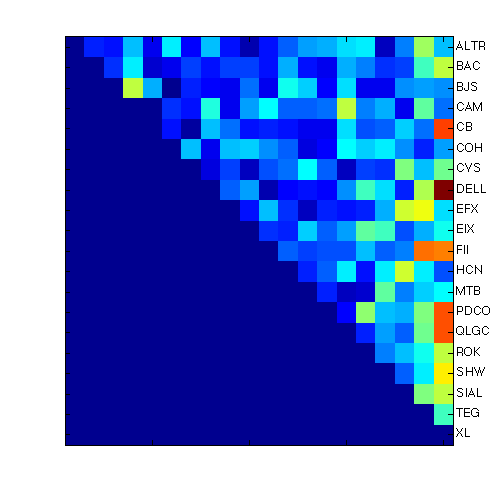
\includegraphics[height=0.18\textheight]{fig/stocks2.png}
  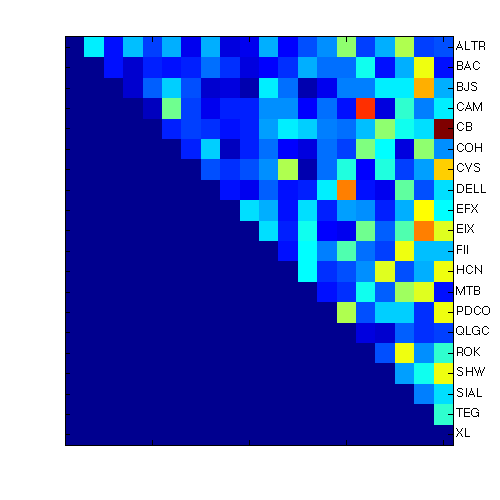
\includegraphics[height=0.18\textheight]{fig/stocks3.png}
  \hspace{4mm}
  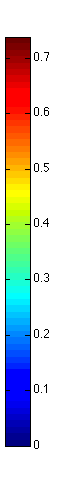
\includegraphics[height=0.18\textheight]{fig/colorbar.png}
  \caption{Heatmaps showing posterior probability of edges in stock network in sequence of 3 weeks.}
  \label{fig:stockResults}
\end{figure*}


\section{Conclusion}
\label{sec:conclusion}

We have derived a time-varying, Bayesian model for inferring the structure of a sequence of Gaussian graphical models. Through experiments on synthetic data we have shown that our dynamic model outperforms static equivalents. We have also demonstrated our method on multiple real-life datasets in order to show its ability to infer network structure in the fields of both finance and genetics. 

Our principal motivation for pursuing Gaussian graphical model structure learning in a Bayesian setting is that generative models allow for flexible specification of dependencies between variables, especially of the dynamics of time-varying graphs. In our DBN, we chose a very simple transition model in which each edge flips on or off with some probability $p$ at every time step. We chose a Beta prior that encouraged the value of the Bernoulli parameters to be closer to 1 in order to incorporate our beliefs that the network structure does not change very much from one time point to the next. However, one could very easily construct a similar DBN with a different transition model in order to encode more complex dynamics. This would be especially useful when applying the method in a setting where the dynamics of the evolving network are well studied and there is ample room for prior knowledge to be incorporated into the model design.

In our experiments, due to run time limitations, we only applied our method to small networks with 12-25 nodes. 
%Furthermore, in our synthetic experiment, we generated a large number of observations at each time point ($n = 100$). 
In many real-world settings, however, there is a need to infer the structure of very large networks (thousands of nodes) using only a small number of observations. One of the main limitations of our method is that its computational complexity does not allow it to scale up to large networks. 
%Furthermore, Figure ? indicates that the performance of our method degrades quickly when we don't have enough data. 

\section{Future Work}
\label{sec:future_work}

In this work, we used synthetic data to show that our model yields better performance on time-evolving networks than a series of static models applied separately at each time point. However, it would also be valuable to compare the performance of our method with that of a discriminative technique for learning the structure of a dynamic network, such as \cite{song2009keller}. We also applied our method to two real datasets for which we don't have a ground truth network on which to evaluate performance. However, if we were interested in analyzing these results further, we could examine individual nodes (e.g. specific genes or stocks) and their neighbors, and try to understand whether the existence of edges coincides with underlying properties of the nodes known to specialists in the relevant field. 



As mentioned earlier, a main direction of future work would be to work on coming up with an inference technique that can be optimized to run much faster, and scale up to much larger networks with thousands of nodes. 

- Try on some artificial systems with complex dynamics, and incorporate this information into the model
- For real-world applications, analyze results in-depth by looking at what genes have edges that change over time and what genes remain consistent, or the same for stock data



\begin{small}
\bibliographystyle{plainnat}
\bibliography{paper_refs} 

\end{small}



\end{document}
